% command for a new time slot
\newcommand{\talkTime}{9:99}
\newcommand{\newTimeslot}[1]{\newpage\renewcommand{\talkTime}{#1}}

% new time slot but without a pagebreak
\newcommand{\newSmallTimeslot}[1]{\renewcommand{\talkTime}{#1}}

% initialise \conferenceDay 
\newcommand{\conferenceDay}{Noday}


% define default page style (cutting marks with page number)
\DeclareNewLayer[background, oddorevenpage, width=125mm,%
height=169mm, contents={%
  \includegraphics{wallpaper/crop-marks.pdf}%
}]{cropmarksevery}
\newpairofpagestyles[scrheadings]{cropmarksstyle}{}
\AddLayersAtBeginOfPageStyle{cropmarksstyle}{cropmarksevery}

% page style for title pages
\DeclareNewLayer[background, oddorevenpage, width=125mm,%
height=169mm, contents={%
  
\includegraphics{wallpaper/front-cover-with-crop-marks.pdf}%
}]{titlelayer}
\newpairofpagestyles[]{titlestyle}{}
\AddLayersAtBeginOfPageStyle{titlestyle}{titlelayer}

% page style for floor plan of S and M building
\DeclareNewLayer[background, oddorevenpage, width=125mm,%
height=169mm, contents={%
  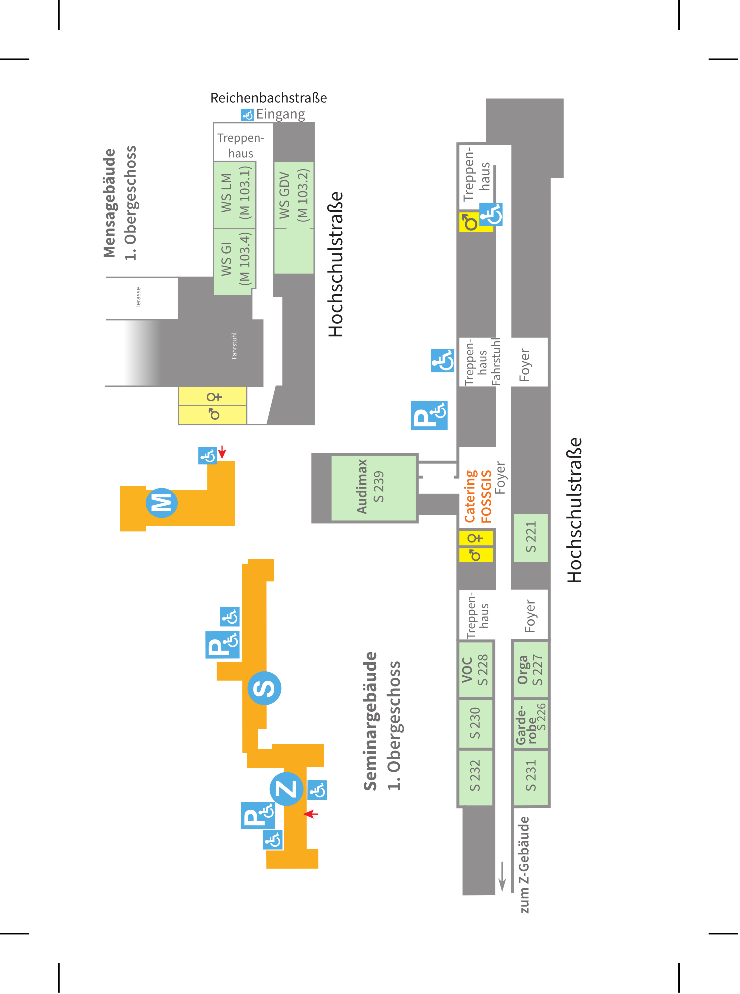
\includegraphics{wallpaper/gebaeudeplaene-s.pdf}%
}]{gebaeudeplanslayer}
\newpairofpagestyles[scrheadings]{gebaeudeplanStyleS}{}
\AddLayersAtBeginOfPageStyle{gebaeudeplanStyleS}{gebaeudeplanslayer}

% page style for floor plan of Z building
\DeclareNewLayer[background, oddorevenpage, width=125mm,%
height=169mm, contents={%
  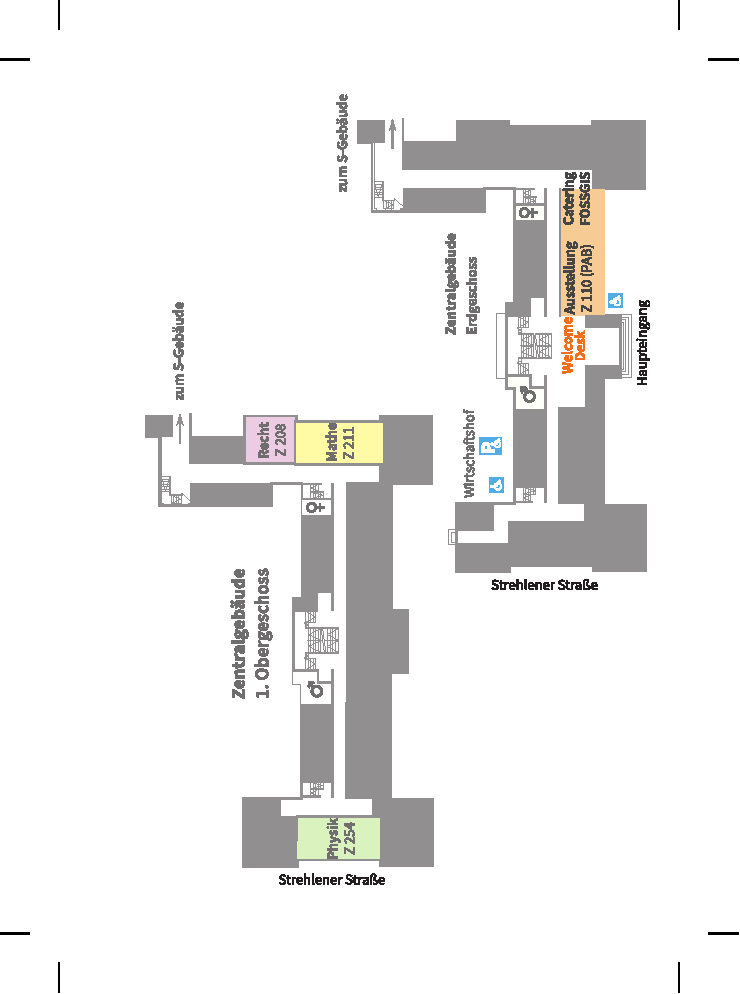
\includegraphics{wallpaper/gebaeudeplaene-z.pdf}%
}]{gebaeudeplanzlayer}
\newpairofpagestyles[scrheadings]{gebaeudeplanStyleZ}{}
\AddLayersAtBeginOfPageStyle{gebaeudeplanStyleZ}{gebaeudeplanzlayer}

% define alias commands for all three days
\def\mittwoch{Mittwoch}
\def\donnerstag{Donnerstag}
\def\freitag{Freitag}

% define Wednesday page style
\DeclareNewLayer[background, oddpage,  width=125mm,%
height=169mm, contents={%
  \includegraphics{wallpaper/mittwoch-ungerade.pdf}%
}]{mittwochungerade}
\DeclareNewLayer[background, evenpage,  width=125mm,%
height=169mm, contents={%
  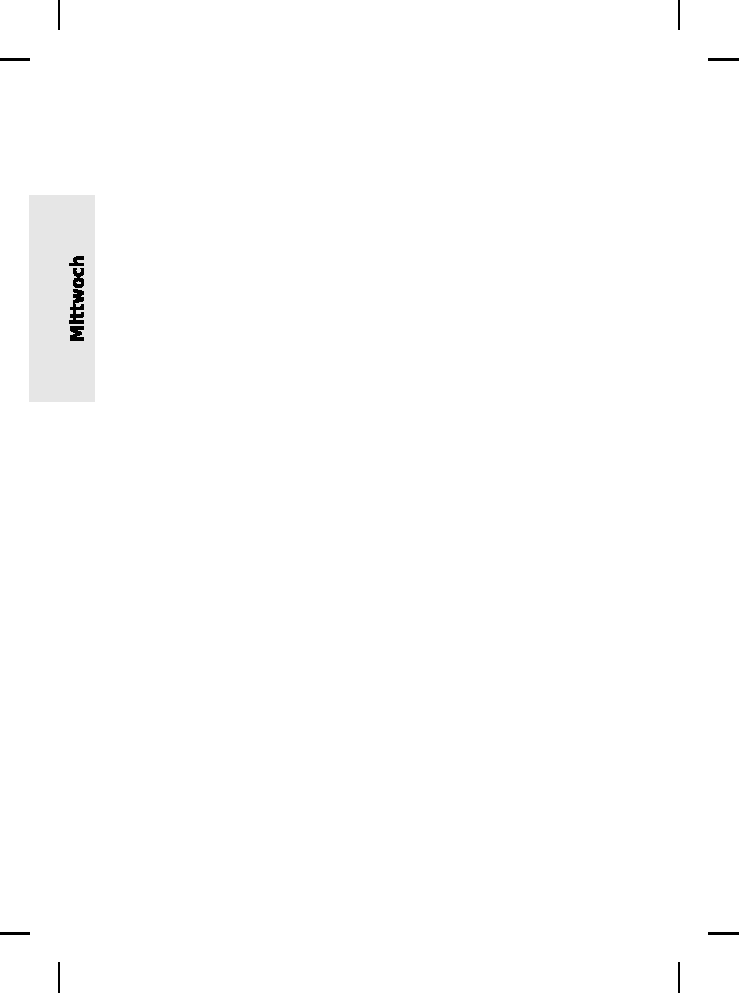
\includegraphics{wallpaper/mittwoch-gerade.pdf}%
}]{mittwochgerade}
\newpairofpagestyles[scrheadings]{mittwoch}{}
\AddLayersAtBeginOfPageStyle{mittwoch}{mittwochgerade}
\AddLayersAtBeginOfPageStyle{mittwoch}{mittwochungerade}

% define Thursday page style
\DeclareNewLayer[background, oddpage,  width=125mm,%
height=169mm, contents={%
  \includegraphics{wallpaper/donnerstag-ungerade.pdf}%
}]{donnerstagungerade}
\DeclareNewLayer[background, evenpage,  width=125mm,%
height=169mm, contents={%
  \includegraphics{wallpaper/donnerstag-gerade.pdf}%
}]{donnerstaggerade}
\DeclareNewLayer[background, oddpage,  width=125mm,%
height=169mm, contents={%
  \includegraphics{wallpaper/donnerstag-ungerade-gedreht.pdf}%
}]{donnerstagungeradegedreht}
\newpairofpagestyles[scrheadings]{donnerstag-tabelle}{}
\AddLayersAtBeginOfPageStyle{donnerstag-tabelle}{donnerstaggerade}
\AddLayersAtBeginOfPageStyle{donnerstag-tabelle}{donnerstagungeradegedreht}
\newpairofpagestyles[scrheadings]{donnerstag}{}
\AddLayersAtBeginOfPageStyle{donnerstag}{donnerstaggerade}
\AddLayersAtBeginOfPageStyle{donnerstag}{donnerstagungerade}

% define Friday page style
\DeclareNewLayer[background, oddpage,  width=125mm,%
height=169mm, contents={%
  \includegraphics{wallpaper/freitag-ungerade.pdf}%
}]{freitagungerade}
\DeclareNewLayer[background, evenpage,  width=125mm,%
height=169mm, contents={%
  \includegraphics{wallpaper/freitag-gerade.pdf}%
}]{freitaggerade}
\DeclareNewLayer[background, oddpage,  width=125mm,%
height=169mm, contents={%
  \includegraphics{wallpaper/freitag-ungerade-gedreht.pdf}%
}]{freitagungeradegedreht}
\newpairofpagestyles[scrheadings]{freitag-tabelle}{}
\AddLayersAtBeginOfPageStyle{freitag-tabelle}{freitaggerade}
\AddLayersAtBeginOfPageStyle{freitag-tabelle}{freitagungeradegedreht}
\newpairofpagestyles[scrheadings]{freitag}{}
\AddLayersAtBeginOfPageStyle{freitag}{freitaggerade}
\AddLayersAtBeginOfPageStyle{freitag}{freitagungerade}

% \setpagebackground selects the page style to be used depending on the current day. Each day has
% its own page style.
\newcommand{\setPageBackground}{ %
  \ifthenelse{\equal{\conferenceDay}{\mittwoch}}{%
    \pagestyle{mittwoch}
  }{}
  \ifthenelse{\equal{\conferenceDay}{\donnerstag}}{%
    \pagestyle{donnerstag}
  }{}
  \ifthenelse{\equal{\conferenceDay}{\freitag}}{%
    \pagestyle{freitag}
  }{}
}


% additional column type for tables
\newcolumntype{Y}[1]{>{\RaggedRight\arraybackslash}p{#1}}

%% length of the title boxes
\newlength{\titleboxwidth}
\setlength{\titleboxwidth}{\textwidth}
\advance\titleboxwidth by -6pt

% command to lay out the title boxes
\newcommand{\setAbstract}[6]{
  % 1. speaker
  % 2. title
  % 3. subtitle
  % 4. abstract (Text)
  % 5. colour
  % 6. room
  %\thispagestyle{scrheadings}
  \setPageBackground
  \setlength\tabcolsep{0pt}
  % \setlength{\fboxsep}{0pt}
  \noindent\fcolorbox{white}{#5}{%
    \parbox{\titleboxwidth}{%
      \noindent\begin{tabu}{X[5L]r}
        \isSpeakerEmpty{#1}{#2}{#6}
        \isSubtitleEmpty{#3}
      \end{tabu}%
    }%
  }%
  %
  \isAbstractEmpty{#4}%
  \vspace{0.5em}% space to the next talk even if there is no abstract
  \setlength\tabcolsep{6pt} % set column padding back to default value
}

% lay out the speaker if there is any
% We assume that there is only a subtitle if the talk has a speaker.
\makeatletter
  \newcommand{\isSpeakerEmpty}[3]{%
    % Arguments:
    % 1. speaker
    % 2. title
    % 3. room
    \@ifmtarg{#1}{%
      \par\noindent\large \sectfont #2% % titel
      &
      #3, \talkTime
      \tabularnewline
    }%
    {
      \emph{#1} % Sprecher
      &
      \talkTime
      \tabularnewline
      {%
        \par\noindent\large \sectfont #2%
      }% % titel
      &
      #3
      \tabularnewline
    }%
  }
\makeatother

% Lay out the subtitle
% has to be a separate function and has to be surrounded by \makeatletter for technical reasons
\makeatletter
  \newcommand{\isSubtitleEmpty}[1]{%
    \@ifnotmtarg{#1}{%
      \multicolumn{2}{Y{\linewidth}}{%
        \vspace{-0.6em}%
        \noindent%
        \bfseries
        \normalsize
        \sectfont #1%
      }
      \tabularnewline%
    }
  }
\makeatother

% Lay out the abstract if there is any
% has to be a separate function and has to be surrounded by \makeatletter for technical reasons
\makeatletter
\newcommand{\isAbstractEmpty}[1]{%
  \ifstrempty{#1}{%
    \vspace{1.5em}%
  }{%
    \vspace{0.5em}\newline%
    #1 \par% % abstract
    \vspace{1.5em}% space to the next talk even if there is an abstract
  }%
}
\makeatother

% define colours
%\definecolor{eins}{cmyk}{0 .18 .06 .10}
\definecolor{eins}{cmyk}{0 .13 .04 .08}
\definecolor{zwei}{cmyk}{.1 0 .17 .05}
\definecolor{hellorange}{cmyk}{0 0.18 0.40 0.03}
\definecolor{audimax}{cmyk}{0.13 0 0.04 0.11}
\definecolor{geoblau}{cmyk}{0.24 .02 0 .01}
\definecolor{dezentrot}{cmyk}{0 .24 0.29 .04}
\definecolor{hellgelb}{cmyk}{0 .02 0.36 0}
\definecolor{hellgruen}{cmyk}{0.10 .0 0.22 0.05}

% abstract at Audimax (S239)
\newcommand{\abstractAudimax}[4]%
{%
  \setAbstract{#1}{#2}{#3}{#4}{geoblau}{S239}
}

% abstract at Mathe (Z211) 
\newcommand{\abstractMathe}[4]%
{%
  \setAbstract{#1}{#2}{#3}{#4}{hellgelb}{Z211}
}

% abstract at Physik (Z254)
\newcommand{\abstractPhysik}[4]%
{%
  \setAbstract{#1}{#2}{#3}{#4}{hellgruen}{Z254}
}

% event at Bärenzwinger
\newcommand{\abstractBaerenzwinger}[4]%
{%
  \setAbstract{#1}{#2}{#3}{#4}{dezentrot}{Bärenzwinger}
}

% abstract at Recht (Z208)
\newcommand{\abstractRecht}[4]%
{%
  \setAbstract{#1}{#2}{#3}{#4}{eins}{Z208}
}

% abstract at a different location
\newcommand{\abstractOther}[5]%
{%
  \setAbstract{#1}{#2}{#3}{#4}{hellorange}{#5}
}

% infobox for workshops (they don't have an abstract in the booklet)
\newcommand{\workshopbox}[3]{%
  % 1. titel
  % 2. speaker
  % 3. Room
  \setlength\tabcolsep{0pt}
  \noindent\fcolorbox{white}{dezentrot}{%
    \parbox{\titleboxwidth}{%
      \noindent%
      \begin{tabu}{X[5L]r}
        \emph{#2} % Sprecher
        &
        \talkTime
        \tabularnewline
        {\noindent\large \bfseries #1}% % title
        &
        #3
        \tabularnewline
      \end{tabu}
    }
  }
  \setlength\tabcolsep{6pt} % set column padding back to default
}

% too long
\newcommand{\tooLong}{Dieser Text ist viel zu lang. Dieser Text ist viel zu lang. Dieser Text ist viel zu lang. Dieser Text ist viel zu lang. Dieser Text ist viel zu lang. Dieser Text ist viel zu lang. Dieser Text ist viel zu lang. Dieser Text ist viel zu lang. Dieser Text ist viel zu lang. Dieser Text ist viel zu lang. Dieser Text ist viel zu lang. Dieser Text ist viel zu lang. Dieser Text ist viel zu lang. Dieser Text ist viel zu lang. }

\newlength{\fboxwidth}

\def\workshopsSection{workshopsSection}
\def\abstractsSection{abstractsSection}

% boxes for text-only advertisement texts by our sponsors
\newcommand{\sponsorBox}[4]{%
  \setlength{\fboxwidth}{\textwidth}
  \advance\fboxwidth by -7.0pt
  \abstractSponsorbox{#1}{#2}{#3}{#4}{\workshopsSection}%
}

\newcommand{\sponsorBoxA}[4]{%
  \setlength{\fboxwidth}{\textwidth}
  \advance\fboxwidth by -10.0pt
  \abstractSponsorbox{#1}{#2}{#3}{#4}{\abstractsSection}%
}

%% store \parindent in separate variable because it is resetted to 0 in parboxes
\newlength{\saveparindent}
\setlength{\saveparindent}{\parindent}

%% box for advertisment by a sponsor
%% 1. logo
%% 2. width of the logo
%% 3. number of required lines of the logo (due to usage of wrapfigure)
%% 4. text
%% 5. Umfeld (\workshopsSection oder \abstractsSection}
\makeatletter
  \newcommand{\abstractSponsorbox}[5]{%
    \setlength{\fboxsep}{4.5pt}%
    \noindent%
    \ifthenelse{\equal{#5}{\workshopsSection}}{%
      \hspace{2.65pt}%
    }{%
      \hspace{-1pt}%
    }%
    \fcolorbox{gray}{white}{%
      \parbox{\fboxwidth}{
        \setlength{\parindent}{\saveparindent}%
        \@ifmtarg{#1}{}{%
          \begin{wrapfigure}[#3]{r}[0pt]{#2}
            \centering\vspace{-1\baselineskip}
            \includegraphics[width=#2]{#1}
          \end{wrapfigure}
        }
  
        \noindent #4
      }%
    }
    \setlength{\fboxsep}{3pt}
  }
\makeatother

% definition of column types for the schedule tables
\newcolumntype{Z}[1]{>{\RaggedRight\arraybackslash}p{#1}}%
\newcolumntype{C}[1]{>{\Centering\arraybackslash}p{#1}}%

% common implementation of typesetting of a session in the tables
\newcommand{\talkInternal}[2]{%
  \textbf{#1}
  \ifthenelse{\equal{#2}{}}{}{%
    \newline\emph{#2}%
  }
}

% macro to typeset a talk in the schedule tables spanning over more than one row:
% usage: \longTalk{rowcount}{title}{speaker}
\newcommand{\longTalk}[3]{%
  &
  \multirow{#1}{\linewidth}{%
    \parbox{\linewidth}{
      %HACK Inserting a \vspace here is a dirty hack but it works.
      \vspace{0.45\baselineskip}
      \talkInternal{#2}{#3}%
    }
  }%
}%

% macro to typeset a talk in the schedule tables spanning over more than one row:
% usage: \talk{title}{speaker}
\newcommand{\talk}[2]{%
  &
  \talkInternal{#1}{#2}%
}%


\newcommand{\workshop}[3]%
{%
  \workshopbox{#1}{#2}{#3}
}%

\newcommand{\otherevent}[1]%
{%
  & \textbf{#1}
}%

\newcommand{\audimaxEvent}[2]%
{%
  &
  \multicolumn{3}{c}{
    \textbf{#1} (Audimax) \par \emph{#2}
  }
}%

\newcommand{\coffeespace}{\vspace{0.4em}}
\newcommand{\workshopspace}{\vspace{0.5em}\\}

% define colors
\definecolor{commongray}{gray}{.9}

% macro for no-video icon
% Argument: height
\newcommand{\noVideo}[1]{%
  
\includegraphics[height=#1]{no-video.pdf}%
}
